\documentclass{dcbl/challenge}

\setdoctitle{Naive Transistor Logic}
\setdocauthor{Stephan Bökelmann}
\setdocemail{sboekelmann@ep1.rub.de}
\setdocinstitute{AG Physik der Hadronen und Kerne}
\usepackage{graphicx}
\usepackage{caption}

\begin{document}

When George Boole applied the mathematical framework to the idea of preposition- and class-logic, he couldn't know, what was going to follow. 
Less than a hundret years later, Claude E. Shannon applied boolean algebra to analyse switching circuits.
This lead to the development of so called logic gates. 
A logic gate can be defined as a binary function, which implements the basic boolean operators of NOT, AND, OR, XOR, etc.. 
In order for us to use them, we should take a brief look in how these gates work. 

\section*{Exercises}
\begin{aufgabe}
    Images \ref{fig:not1} and \ref{fig:not2} illustrate the implementation of a naive NOT-gate.
    Reproduce this circuit in Falstad's Circut Simulator and describe how it works.\\\\
    \vspace{1cm}
    \noindent 
    \begin{minipage}{.5\textwidth} 
    \centering
    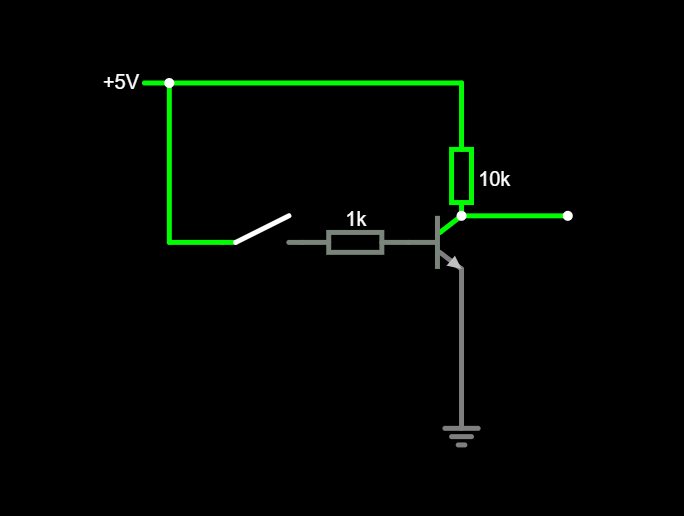
\includegraphics[width=.9\linewidth]{not1.png} 
    \captionof{figure}{Input is 0} 
    \label{fig:not1}
    \end{minipage}
    \begin{minipage}{.5\textwidth}
    \centering
    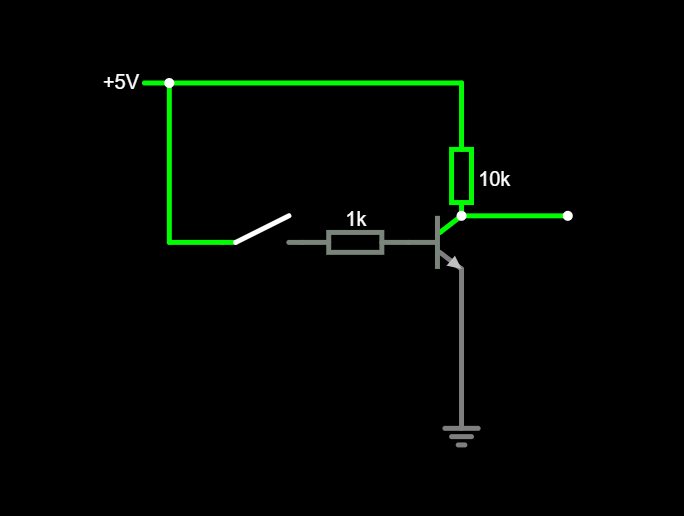
\includegraphics[width=.9\linewidth]{not1.png}
    \captionof{figure}{Input is 1}
    \label{fig:not2}
    \end{minipage}
\end{aufgabe}

\begin{aufgabe}
    With this first example in mind, implement a logic gate, that inverts the output of the NOT-gate once again.
\end{aufgabe}

\begin{aufgabe}
    Add another switch to the design and that implements the boolean OR-operator.
    Can you come up with a solution for a NOT(OR)-gate as well? 
\end{aufgabe}

\begin{aufgabe}
    Implement a AND-gate as well as a NAND-gate.
\end{aufgabe}

\section*{Annotations}
\begin{enumerate}
    \item Claude E. Shannons Masterthesis: "A symbolic analysis of relay and switching circuits" \url{https://doi.org/10.1109/T-AIEE.1938.5057767}
    \item Falstad's Circut Simulator: \url{https://www.falstad.com/circuit/}
    \item \url{https://en.wikipedia.org/wiki/Boolean_algebra}
    \item \url{https://en.wikipedia.org/wiki/Logic_gate}
\end{enumerate}

\end{document}
